\chapter{Results}

The evaluation of performance differences is of utmost importance since it also influences the reliability of claims that refined architectures like the Attentive Fingerprint are capable of learning generalizable knowledge about molecular structures (and, because such knowledge is crucial for accurate predictions, outperform previous models).

Similarly, it could be insightful to check whether the same difference ranking occurs for different runs and, in case of different splits, and whether similar molecules – or the same molecules in case they appear multiple times in the test set – behave also similarly.

A thorough comparison of all these schemes is beyond the scope of this work.
In some cases, probably optimal solutions are thus overlooked and one should generalize with caution.

The focus was rather on two related questions:

\begin{enumerate}
	\item Which factors can help explain the differing results in previous work?
	\item Are there at least some basic guidelines for deciding which method is better performing?
\end{enumerate}

This issue is very common, compare e.g. the results in \cite{Jiang.2024,Liu.2025}.

\subsection{Preliminary remarks}

If the main reason for an inferior performance of GNNs compared to Morgan Fingerprints is overfitting, whereas the ability to discern substructures is equal, it should be possible to compensate for these detrimental factors by techniques like dropout or altered training data and achieve at least equal performance.

It should be further stressed that the differences in performance presented are usually rather small.
In this regard, it is also a central goal to assess which architectural decisions really matter.

After a first investigation, it turned out that the datasets differ highly in difficulty: Whereas for some (e.g. the ESOL dataset), all architectures achieve 'good' results, for other ones even a positive correlation between true and predicted values is hard to achieve; in some cases, suboptimal parameters lead to horizontal curves for regression tasks.


In particular, one should also point at the danger of biases in the datasets itself.

In principle, it could be that the GCN architecture produces the same output for different molecules. However, with respect to the training task, this can be appropriate (for a binary classification task, it would suffice to map all molecules to exactly two numbers etc.)


Therefore, in cases for which a modified architecture was used, but hyperparameter optimization was not done anew, one should be aware that in principle a further improvement could be possible. (This is in particular true for extended, more complicated architectures, like the combining of layers.)


Analogously, for classification tasks, one has to check whether the ratio between the classes affects molecular fingerprints differently than graph representations.


(Most of the datasets were used in other studies evaluating either the performance of Morgan fingerprints or graph representations; however, due to the problems elaborated on above, a comparison was impossible.)

A major incentive for the application of very diverse datasets was the detection of differences in performance.


The main goal was to get a rough overview of whether or what differences and size there are between the architectures.

In some cases, default values are omitted for a clearer representation (e.g., the default for Jumping Knowledge is ‘None’, equally for dropout and normalization layers, and also usually no frozen layers are applied).

\section{Comparison of embeddings and substructures on 'toy examples'}

In principle, it should therefore be possible to replicate the feature vector generated by the Morgan algorithm by using GNNs. 

Again, it has to be stressed that the maximizing of expressivity, i.e. the ability to distinguish between input graphs, is not a conditio sine qua non for success in the molecular property prediction tasks. In fact, it can be a hindrance; in particular for binary classification tasks, a mapping onto two different feature vectors would be sufficient.

One possibility is to ‘train’ the network with all weights frozen.
Comparison with the trained version shows whether trained parameters lead to a diminished differentiation of graphs (which is not necessarily accompanied by a drop in performance, but can even be beneficial).

(For reasons of efficiency, it cannot be recommended to use such a neural network in practice; in almost every scenario, the computation of the fingerprints is much faster and less resource-intensive than the instantiation – or even training, which in case of frozen layers can be partly ignored – of a neural network.)


RdKit also supports the computation of rooted fingerprints: Instead of one fingerprint for the full molecule, for specific atoms all substructures are outputted (in case of the Morgan fingerprint, this means all substructures of the specified radius with the selected atom as central atom).

Summing up of all rooted substructures should yield a fingerprint equivalent to the molecule fingerprint; however, there will be substructures counted multiple times.


number of unique nodes per embedding

\section{Hyperparameter optimization}

If not stated otherwise, in the boxplots all information given before 'opt. hyperparameters' indicates fixed parameters (this is important since parameters to be optimized in some runs are treated as fixed in other ones, e.g. Jumping Knowledge).

\section{Inter- and intra-run variance}

To illustrate this problem, for the ESOL dataset the variances for ten runs on the same split (i.e. only the random seed changes, train and test data are identical), and on ten different splits for the optimized parameters are shown.
To disentangle variance between runs on the same data and variance due to different splits, 10 runs of the same architecture with the same data were performed (so only the random seed has changed).
As one sees, even for the same data differences between runs are considerable.


\section{Results for specific datasets / General outcome}

For most datasets, a radius of 2 in combination with a fingerprint size of 2048 performs best. This is in line with the results in \cite{Deng.2023} and \cite{Stepisnik.2021}. Similarly, for GNNs, more than one or two layers usually do not provide optimal results.
(For GINs, the activation function makes a huge difference.)

Only for datasets / splits which are very difficult (partly giving rise to performance hardly better than a random classifier), higher radii or layer numbers are selected by hyperparameter optimization.

It must be noted that due to the classification layer the evaluation becomes much more complex:
In particular, there are optimal combinations with a rather complex, expressive graph architecture and a thin final classifier as well as such ones with a small graph part and a final classifier consisting of multiple dense layers consisting of many neurons.


In the setting with one layer of the same size as the graph output channels, dropout has rather high (e.g. 0.15, in same cases 0.5) values. Usually, a more compact classification layer is used.

\subsection{ESOL}

\begin{figure}
    \centering
    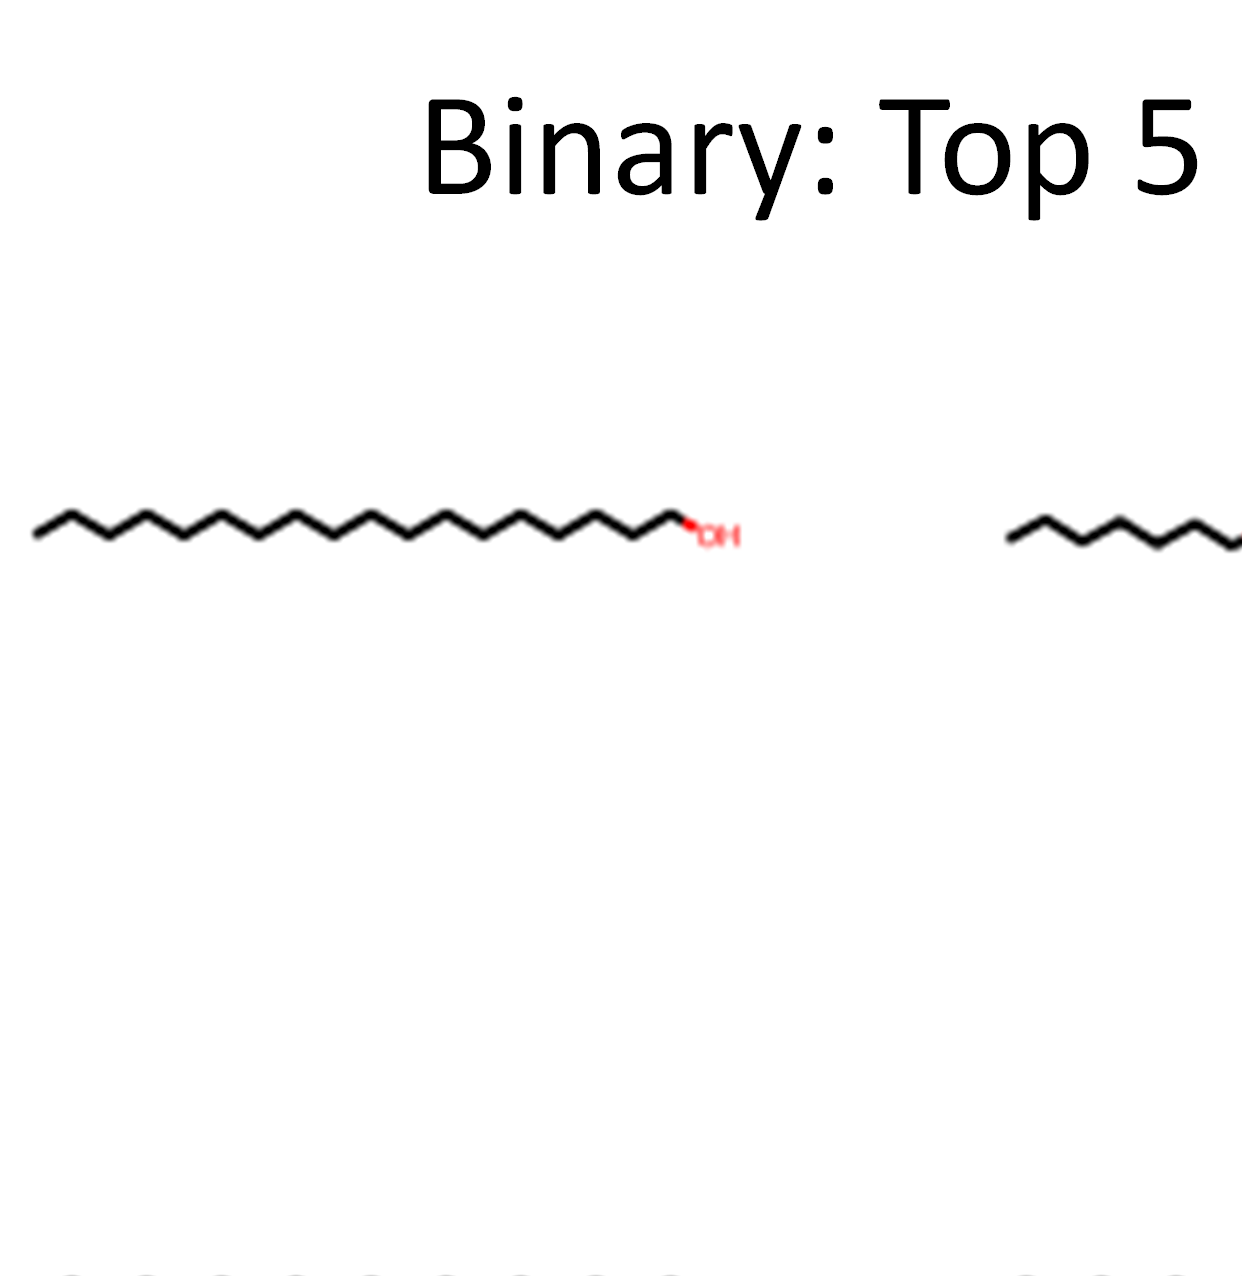
\includegraphics[width=0.25\linewidth]{binary_count_similarity_esol.png}
    \caption{Molecules with top simliarity / ESOL dataset}
    \label{fig:binary_count_similarity_esol}
\end{figure}


\begin{figure}
    \centering
    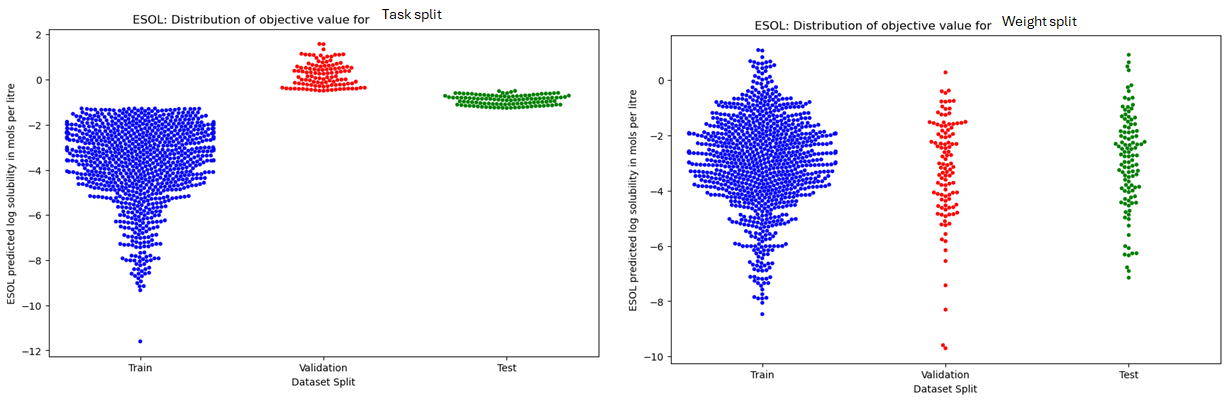
\includegraphics[width=1.15\linewidth]{weight_task_esol.png}
    \caption{Distribution for Task and Weight split on the ESOL dataset}
    \label{fig:weight_task_esol}
\end{figure}


These differences on the task split call for further explanations.



\begin{figure}
	\centering
	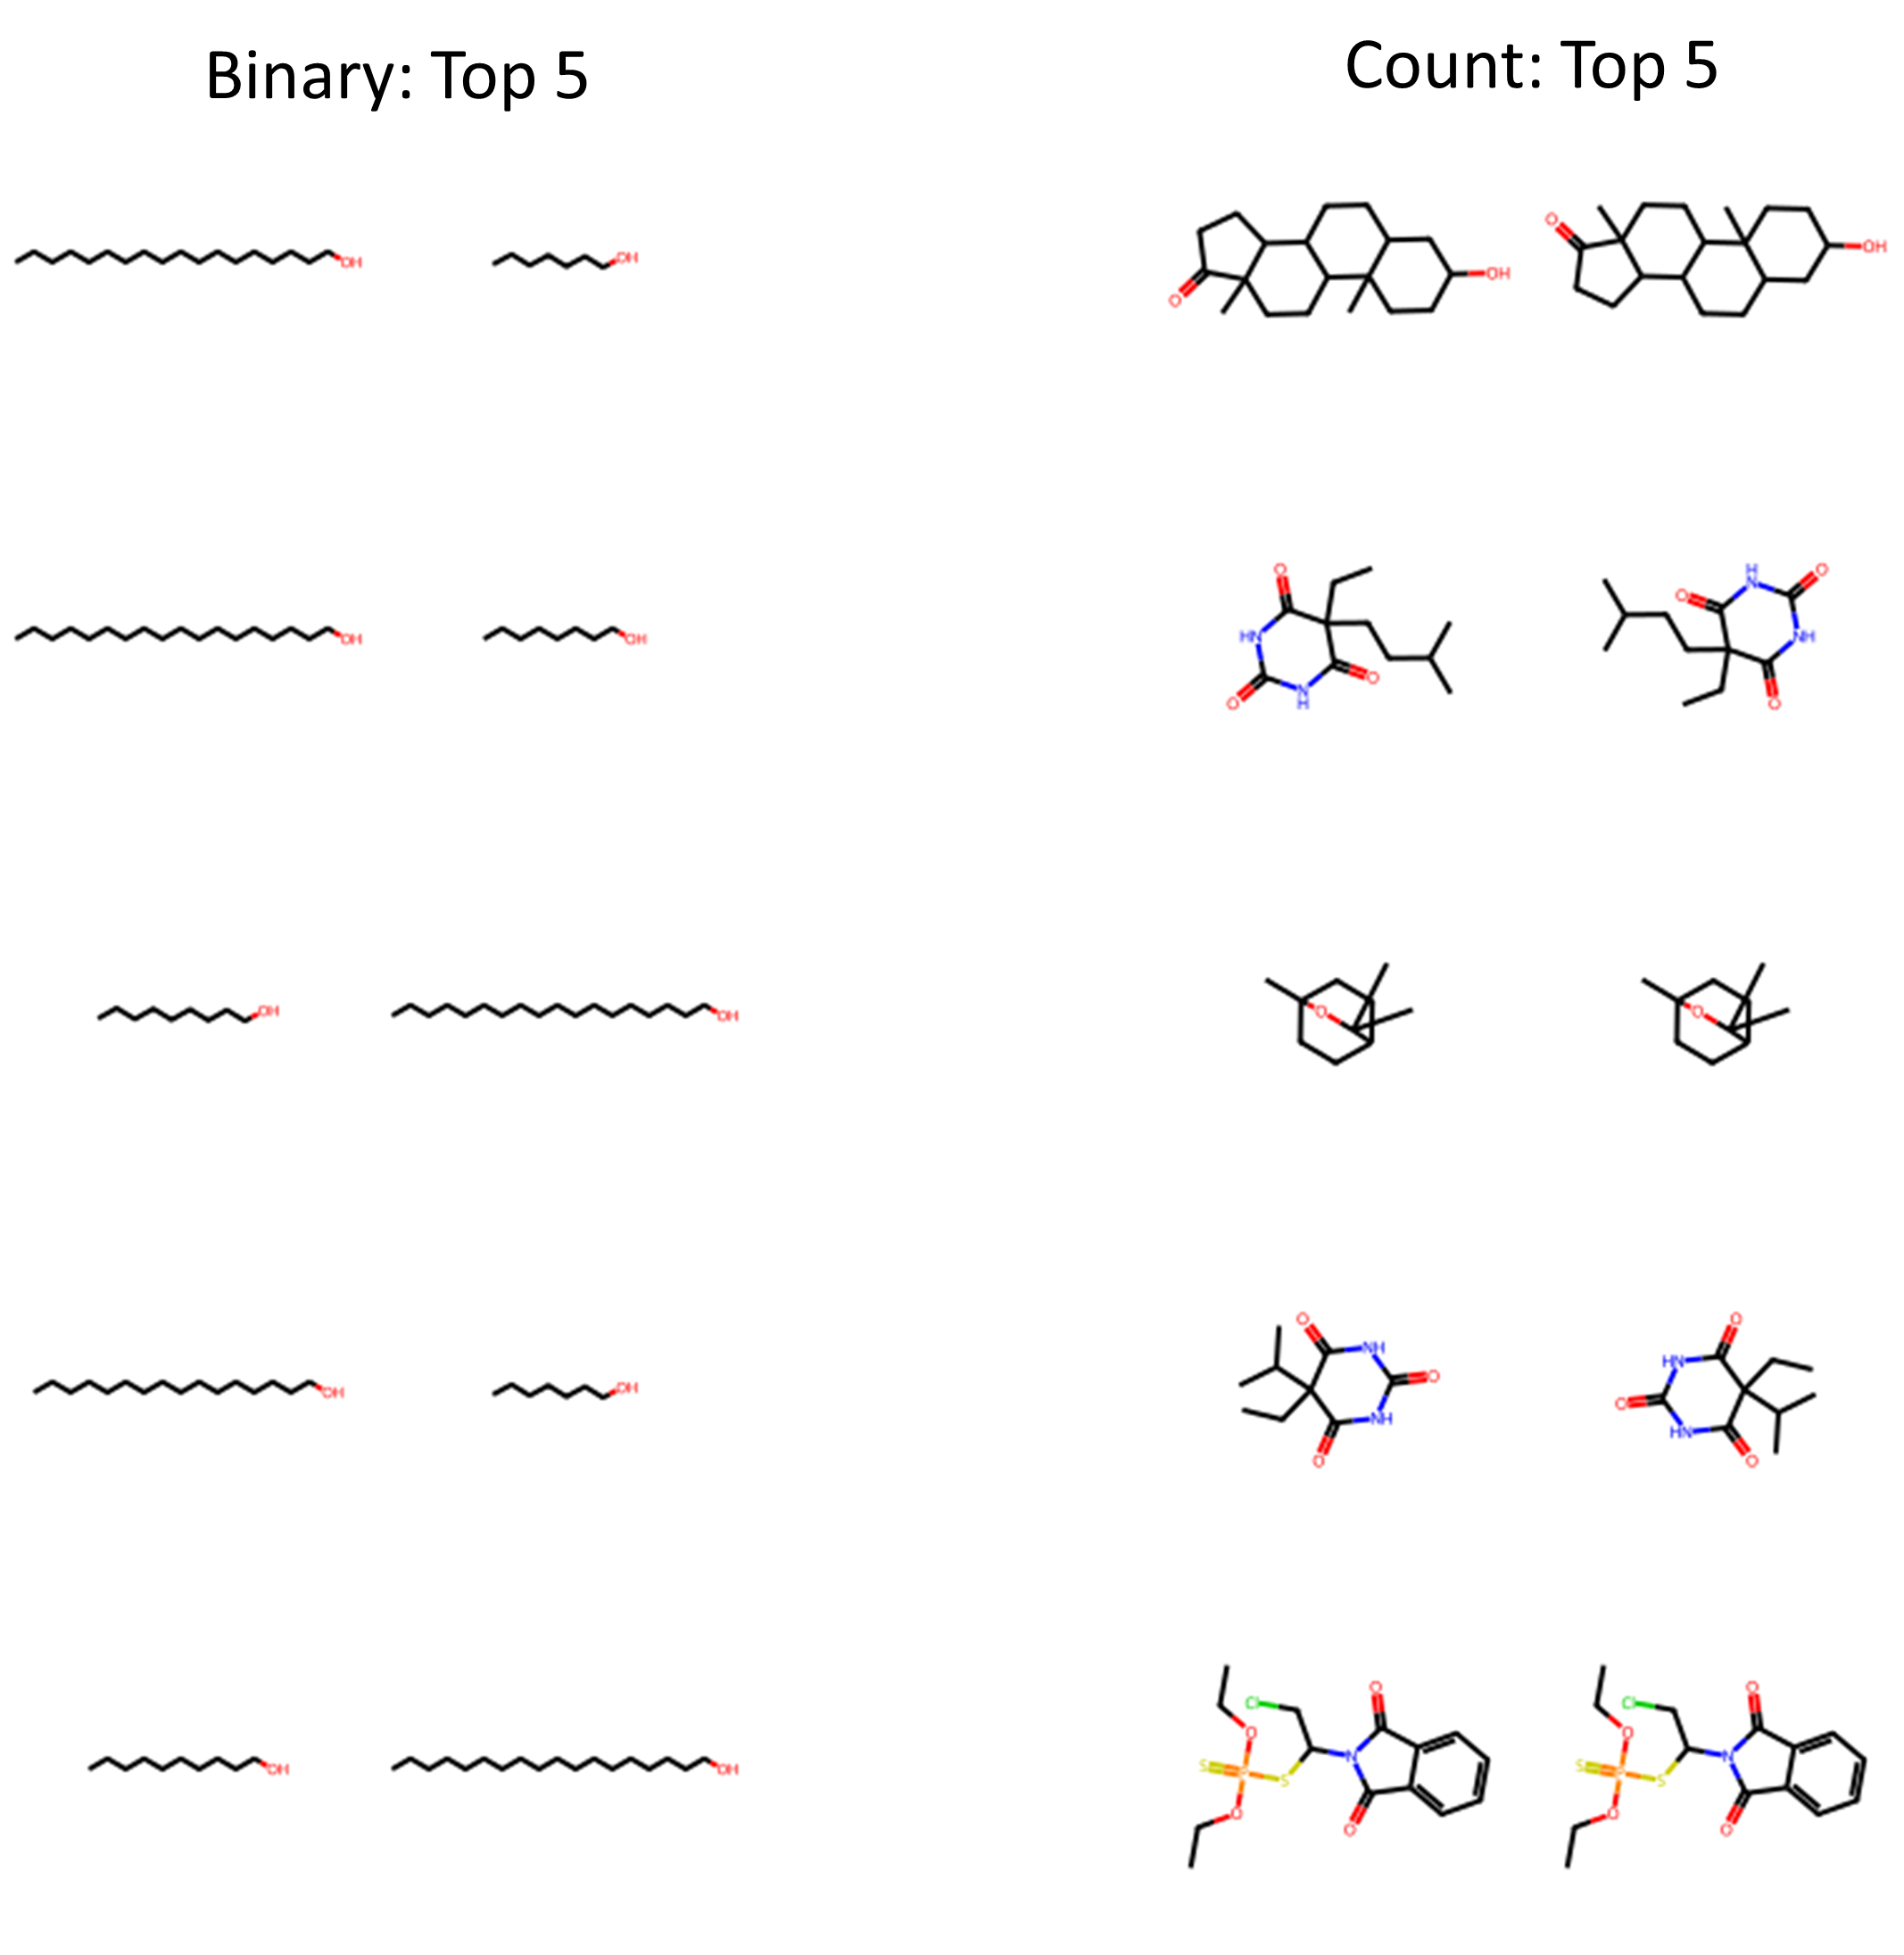
\includegraphics[width=1.15\linewidth]{esol_top5_similarity_binary_count.png}
	\caption{esol_top5_similarity_binary_count}
	\label{fig:esol_top5_similarity_binary_count}
\end{figure}

\ref{fig:esol_top5_similarity_binary_count} clearly shows this effect.


\subsection{BACE}

On this classification task, for many splits classical fingerprints combined with a dense layer perform better than GIN or GCN models.

\subsection{Lipophilicity}

Similarly to the ESOL dataset, an impaired performance of binary Morgan fingerprints in comparison to count-based versions is discernible on the Lipophilicity dataset trained with L1 loss function; however, the difference is rather small.
Interestingly, GINs show a significantly smaller L1 error.
The investigation of the variance shows an even more pronounced difference between Morgan fingerprints and GINs.

\begin{figure}
    \centering
    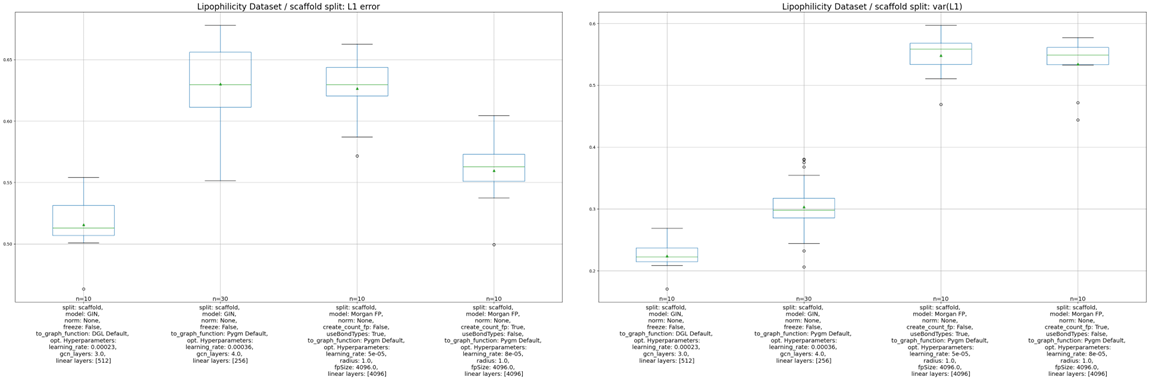
\includegraphics[width=1.00\linewidth]{lipophilicity_res1.png}
    \caption{Lipophilicity dataset: Mean and variance of L1 error}
    \label{fig:lipophilicity_res1}
\end{figure}

Lipophilicity on Task Set!

\subsection{Size and classifiers on the ZINC dataset}


\begin{landscape}
    \centering
    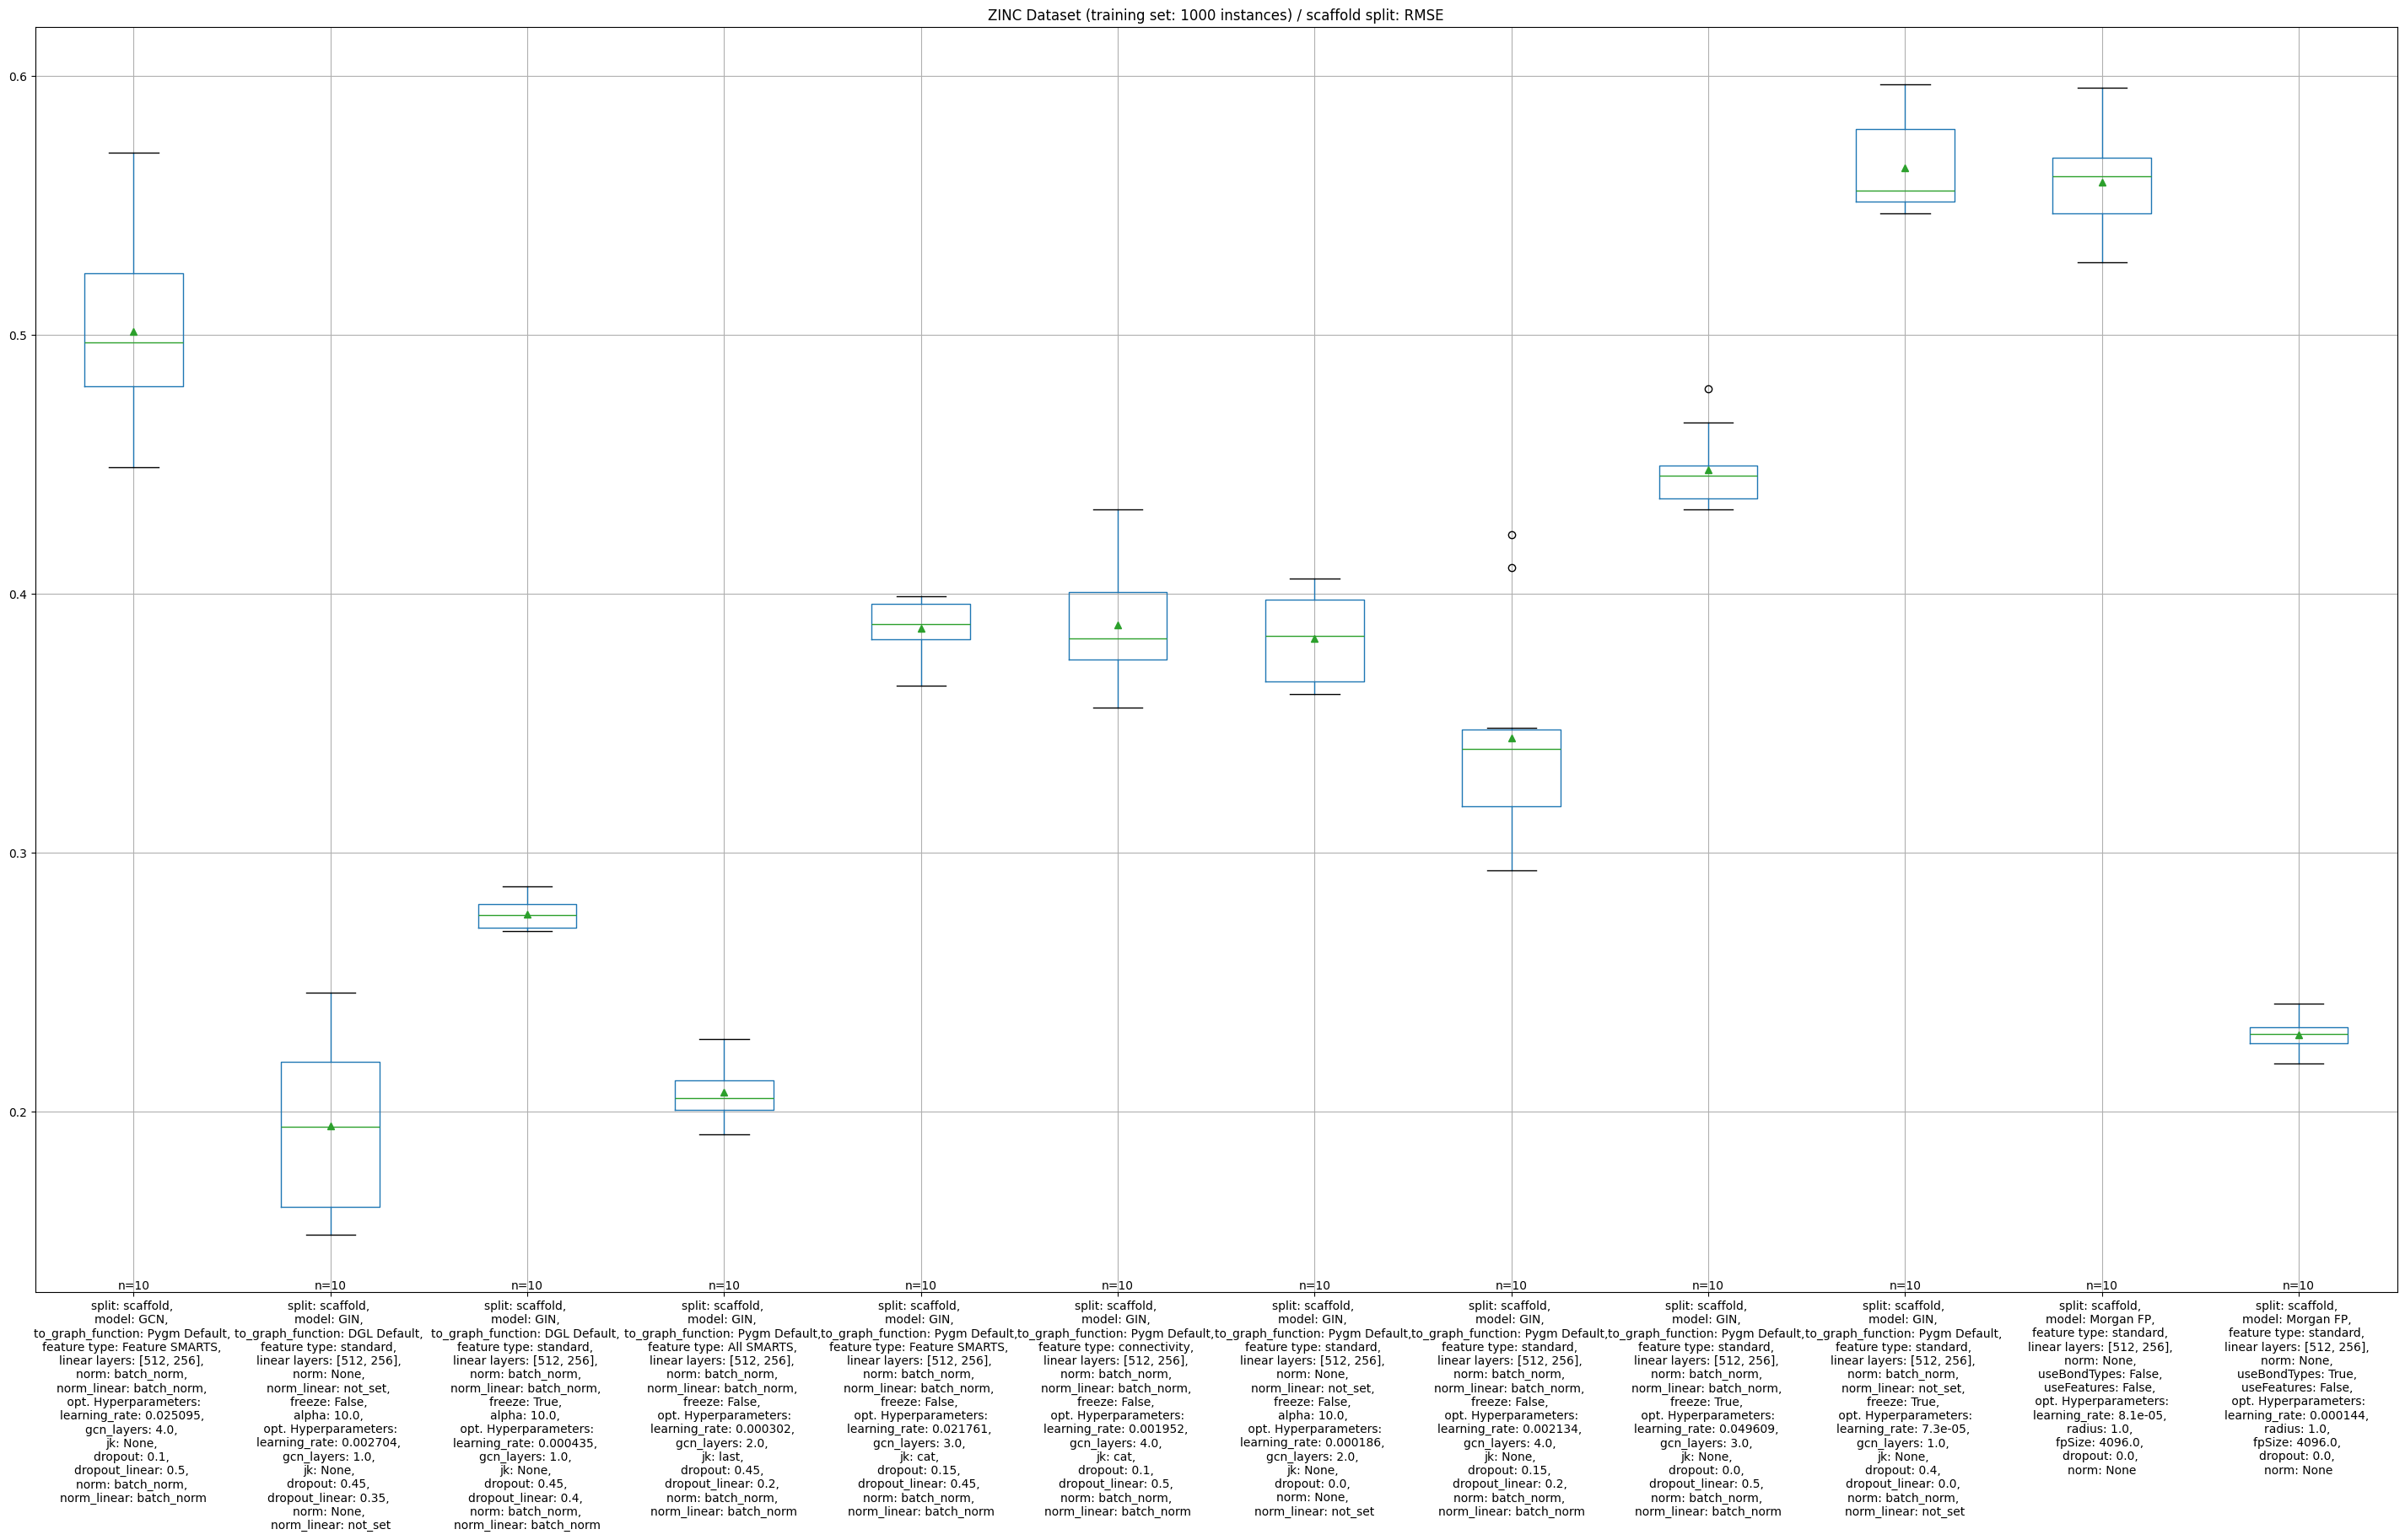
\includegraphics[width=1.05\linewidth]{zinc_1000_scaffold_all1.png}
    \caption{Results for ZINC (1000 training instances) hyperparameter optimization}
    \label{fig:enter-label}
\end{landscape}

Again, frozen parameters with batch normalization perform far worse. Thus a more detailed comparison between such runs with and without batch normalization is advisable.

Interestingly, in this case the Scaled Sigmoid activation function with a high alpha (inducing almost step-function like behaviour) performs best.



It is also one of the rare occasions in which one GNN architecture (GCN) apparently performs much worse than another one (GIN); however, it would be necessary to check this for different feature set configurations.




The enormous size of the ZINC dataset allows for a systematic investigation.
For the ZINC dataset, one could, e.g., use subsets of
500, 1000, 5000, 10000 and 20000 data instances in the training set.

However, linear regression provides almost equally good results.


\subsection{LIT-PCBA dataset}

The LIT-PCBA dataset poses extraordinary challenges due to class imbalance and the creation of the split (see methods).


For this dataset, also an additional run was done.

\subsection{Activity Sets}

The Dopamine dataset is extremely small.

For HERG, much more data is given, leading to a much longer training time.


\section{Influence of the final classifier layer}

In particular, since previous results have shown that this relation is complex, the impact of the final classifier layer has been studied: A richer, more expressive graph representation possibly performs better with a more compact classifier, whereas a small graph readout perhaps needs a bigger (in terms of the number of layers as well as the number of neurons per layer) MLP to extract meaningful features.





Hyperparameter optimization and the set up of the models aimed at maximal flexibility and full control over all parameters. For instance, the values for dropout and batch norm can be applied independently for the GNN part and the subsequent classifier


Interestingly, even with batch norm usually considerably high dropout values (for the graph layers as well as for the dense classifier) are chosen.

In principle, the learnable parameters should not change the ability to discern between molecules and substructures, but the task.
This also implies that a very shallow, simple final classifier leads to greater differences between frozen and learnable parameters.



\section{Splitting-related effects on performance}

In line with expectations, errors are in particular high for values at the margins of the distribution.

For selected datasets, the effect of splitting was investigated.

It should be noted that in previous analyses this was usually not done: Random and scaffold splits were mostly performed, but it was not checked how these split techniques effectively alter the data sets and whether they indirectly cause a task split, i.e. a split concerning the distribution of the objective value.

Fig. \ref{fig:weight_split_esol} and \ref{fig:weight_split_esol_var_mse} show results for 30 runs on the same weight split (so again intra-run variance is measured).
One sees that the variance (although only the random seed has changed) are even much more pronounced than for the random split.

\begin{figure}
    \centering
    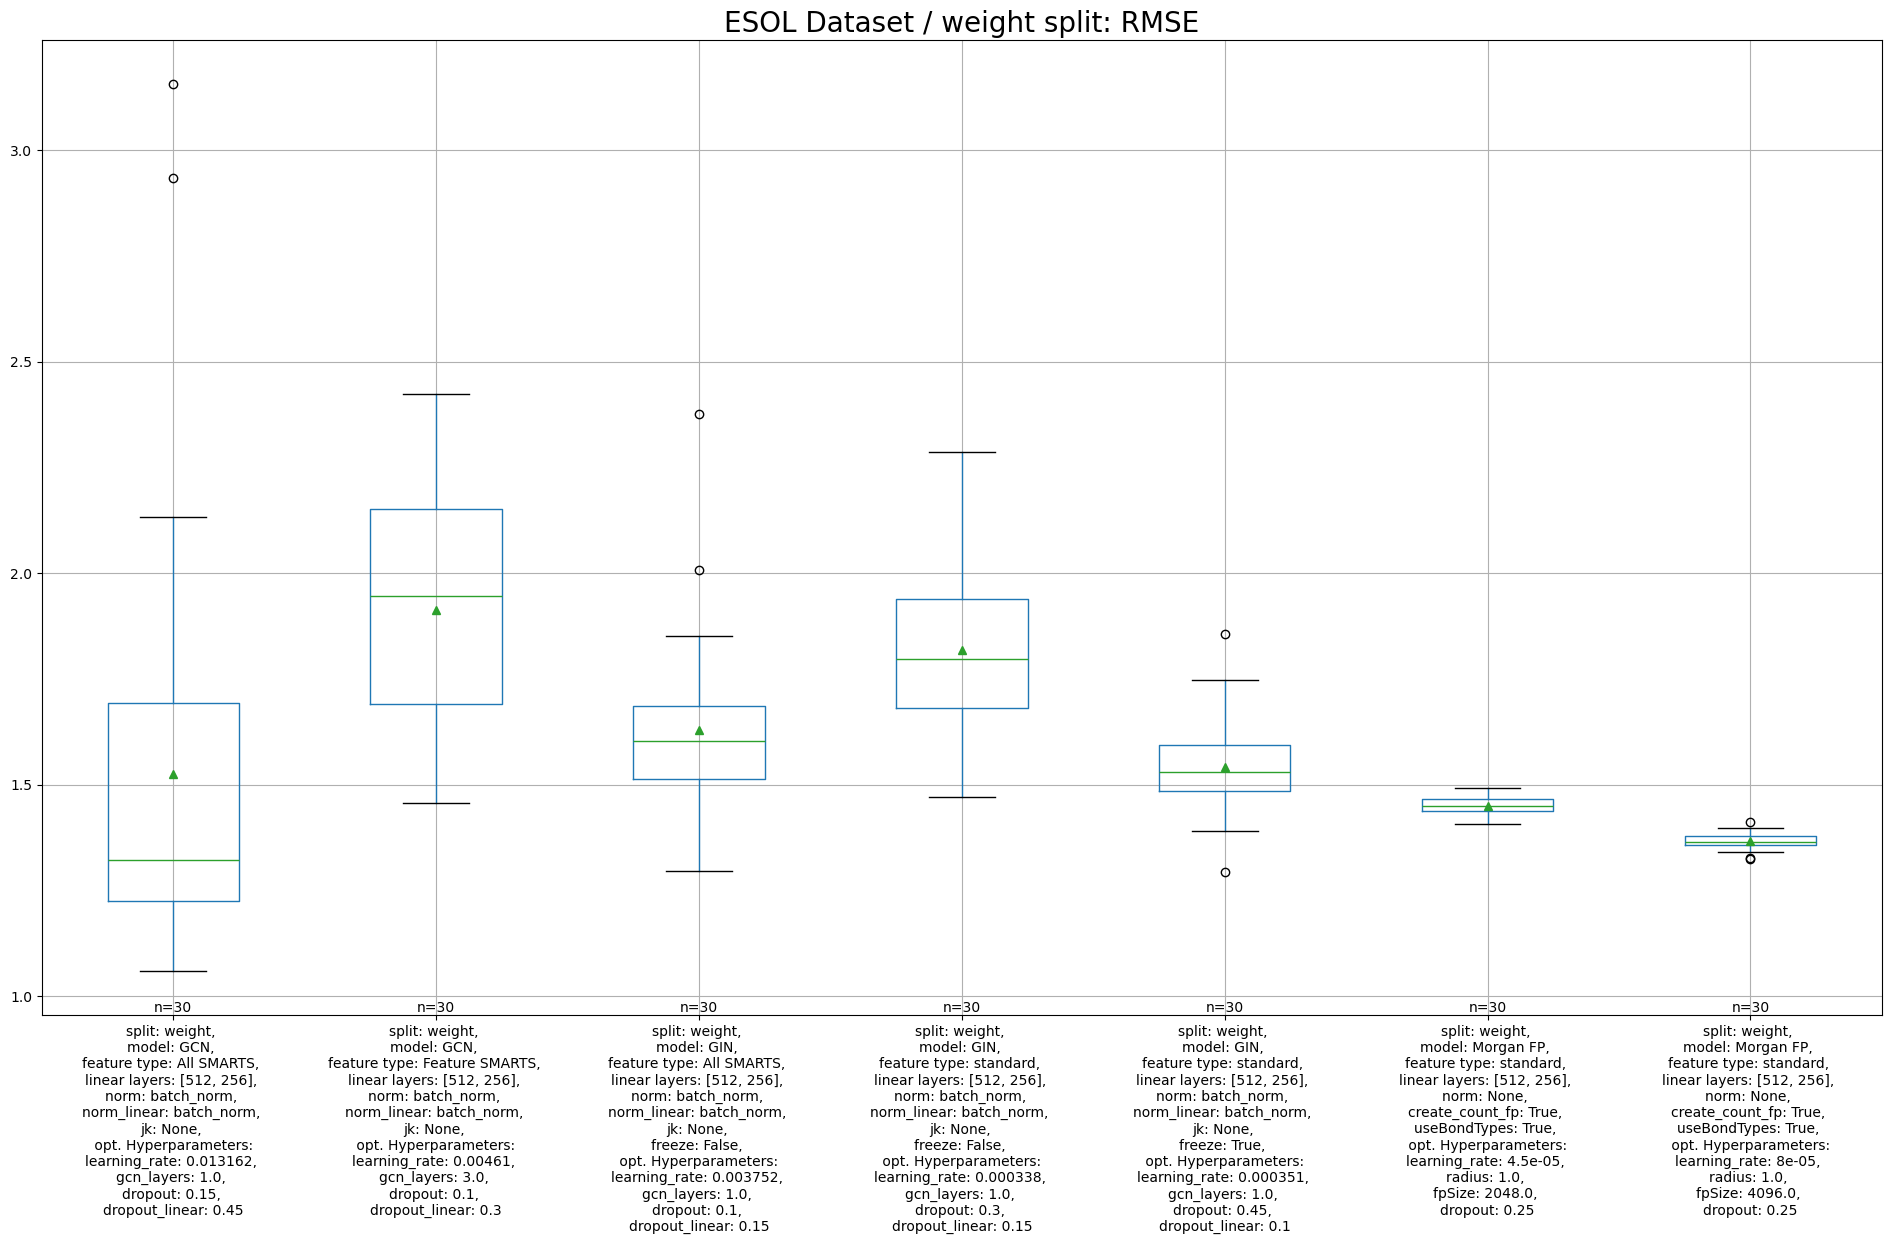
\includegraphics[width=1\linewidth]{weight_split_esol.png}
    \caption{Boxplot three and four as well as five and six show two independent runs with hyperoptimization. The differences in terms of performance as well as found hyperparameters highlight the problems outlined above again. However, the optimized parameters are nonetheless very similar for all architectures; one (or max. two) GNN layers seem to be optimal.}
    \label{fig:weight_split_esol}
\end{figure}



\begin{figure}
    \centering
    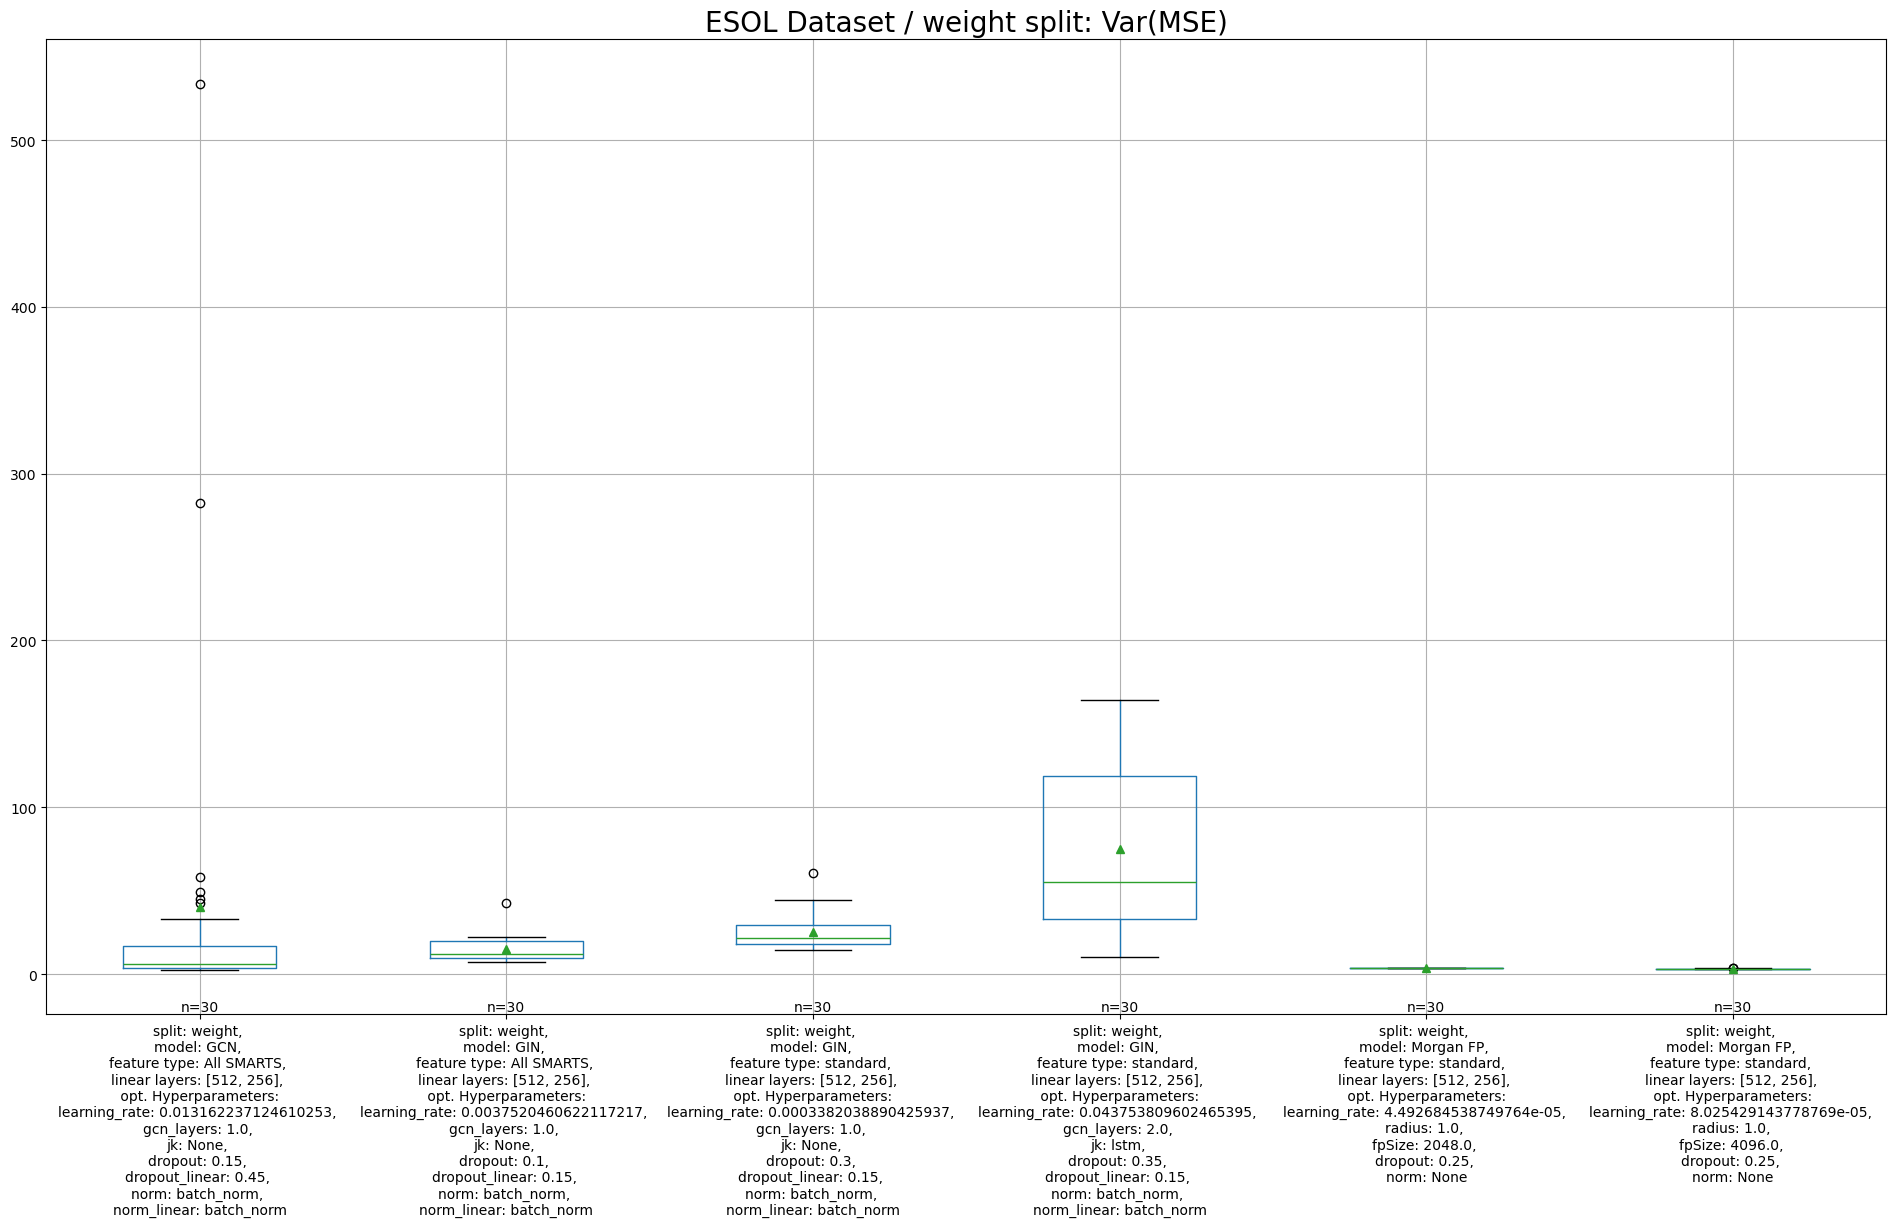
\includegraphics[width=1\linewidth]{weight_split_esol_var_mse.png}
    \caption{Enter Caption}
    \label{fig:weight_split_esol_var_mse}
\end{figure}

Interestingly, it seems that in this case the GIN with frozen layers even performs slightly better.

The combination of all SMARTS strings (the original version from Gobbi and the RDKIT Feature Fingerprint features) give the lowest mean error.


\begin{figure}
    \centering
    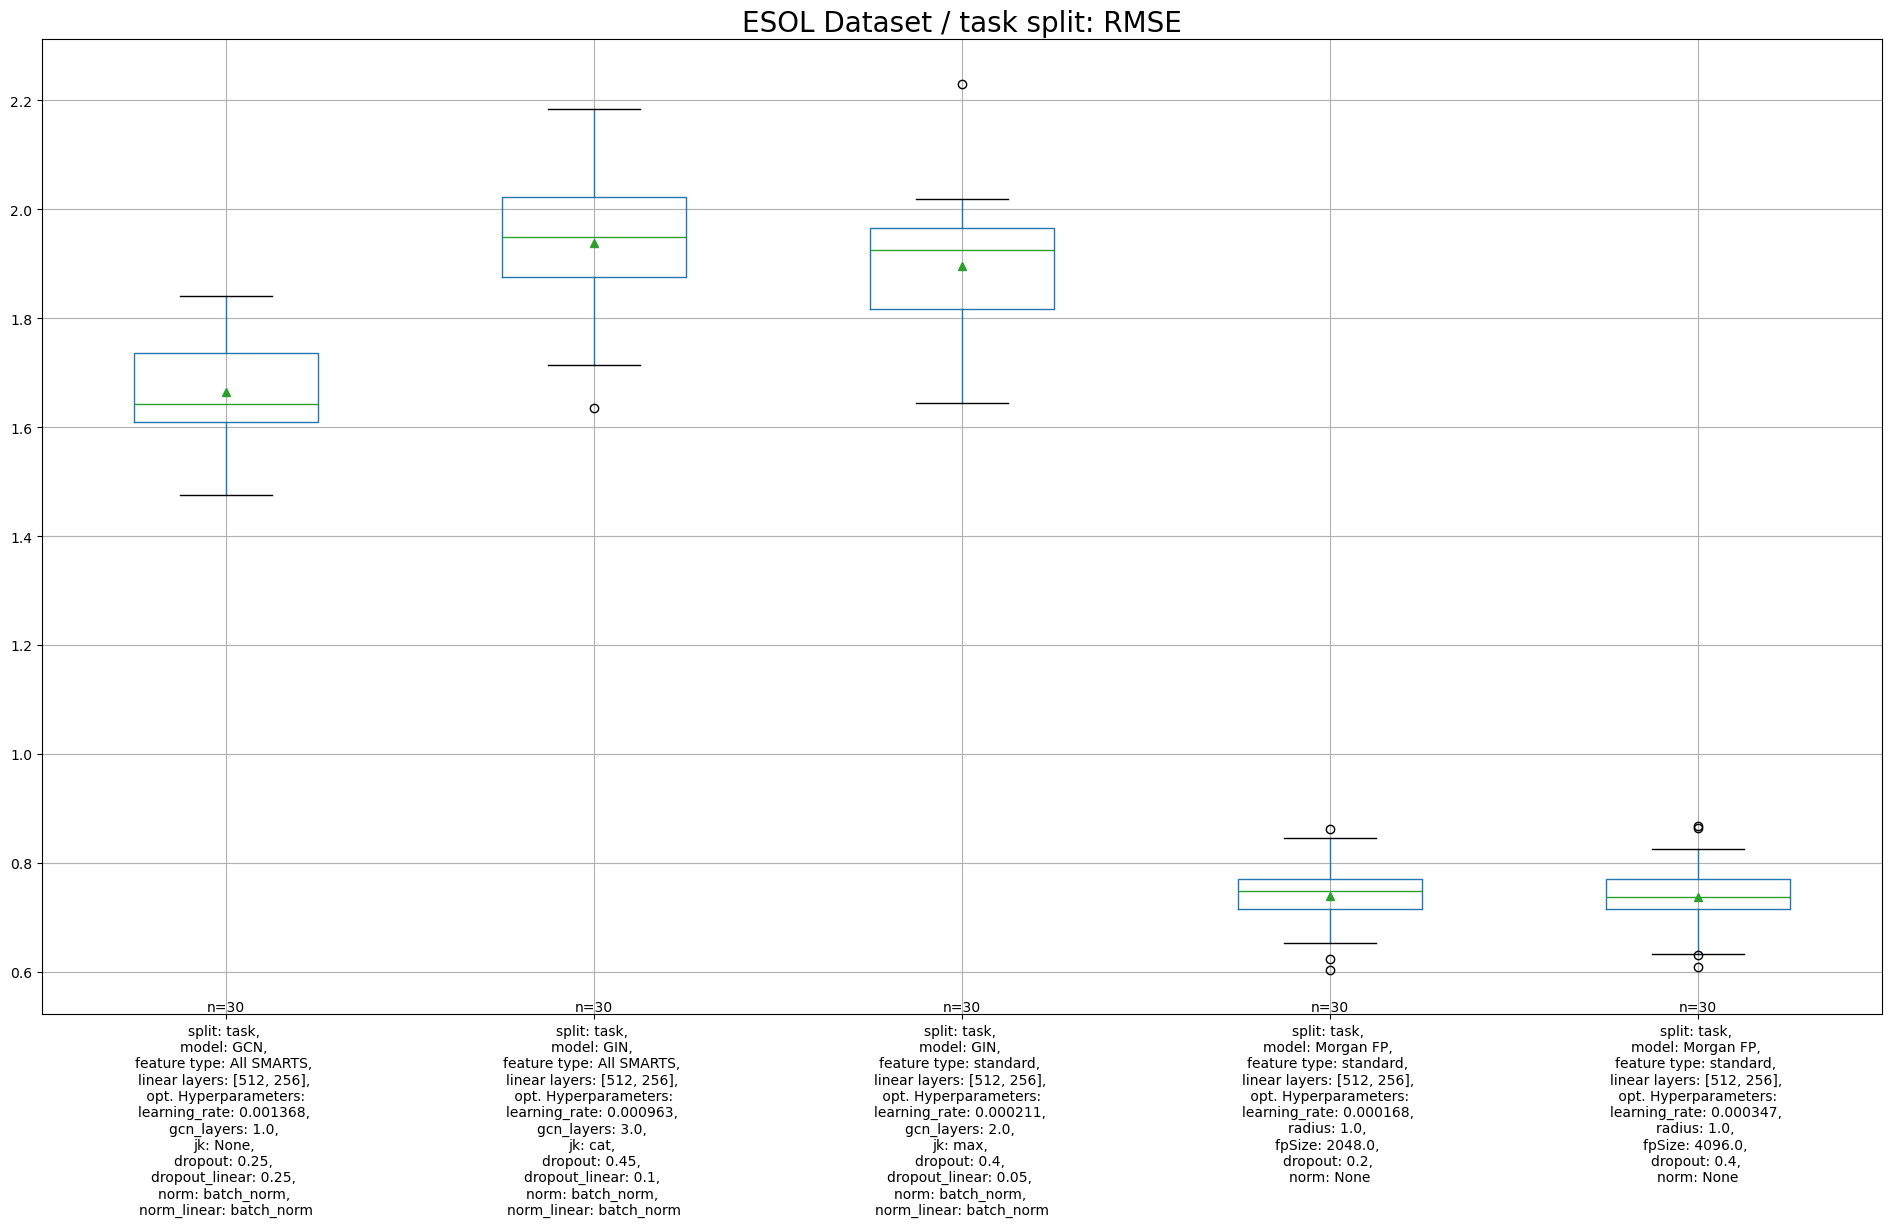
\includegraphics[width=1\linewidth]{task_split_esol.png}
    \caption{Task Split on the ESOL dataset: GCN, GIN and Morgan FP architecture; two runs for Morgan FP}
    \label{fig:task_split_esol}
\end{figure}

\begin{figure}
    \centering
    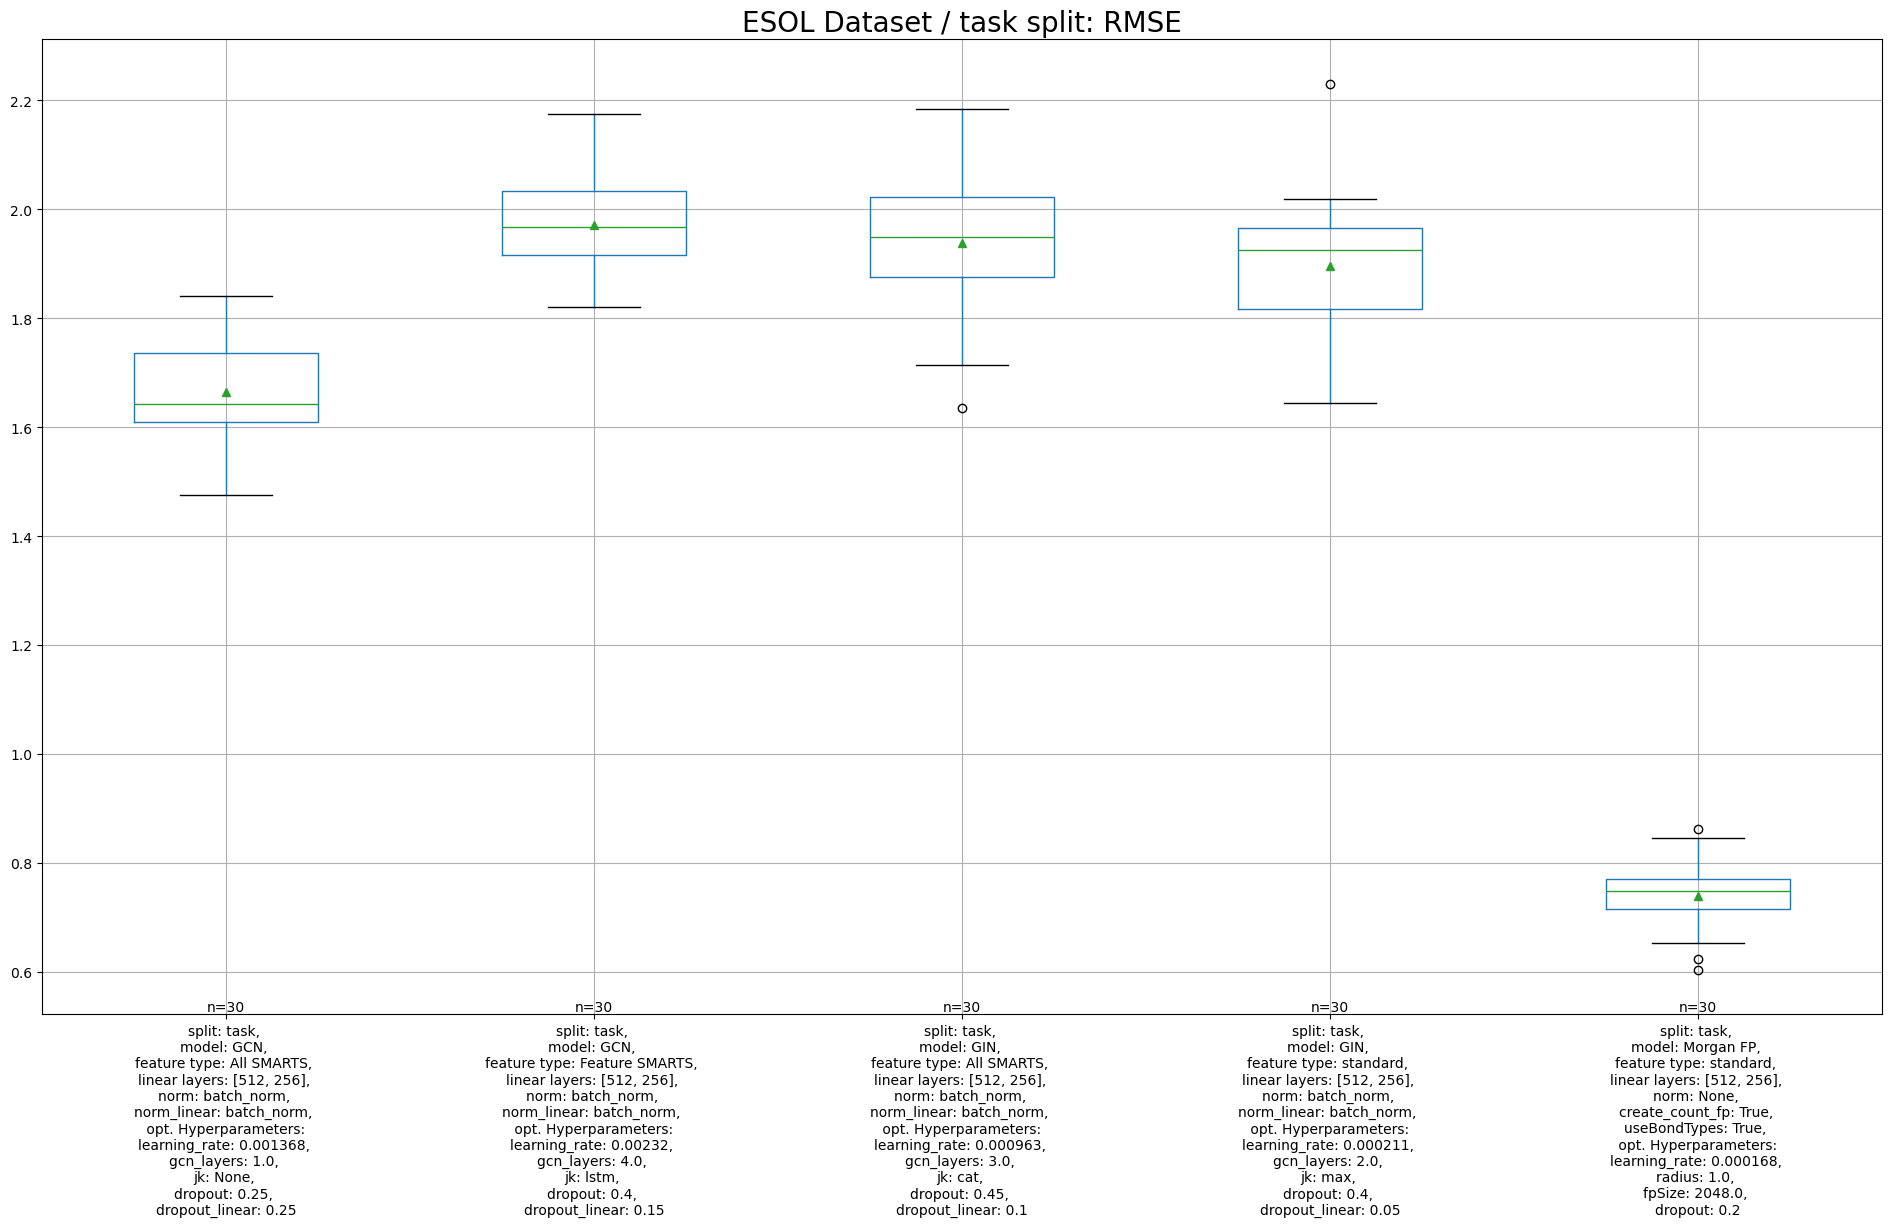
\includegraphics[width=1\linewidth]{task_split_esol_5plots.png}
    \caption{Task Split on the ESOL dataset: GCN, GIN and Morgan FP architecture}
    \label{fig:task_split_esol_5plots}
\end{figure}

For the task split, there are dramatic differences (see fig. \ref{fig:task_split_esol}). Molecular (Count) Fingerprints show a much lower RMSE than graph representations. 


For the splits which reveal tremendous differences between Morgan Fingerprints and GNNs (i.e. task and weight splits), the performance using a combined architecture is of special interest.
On the one hand, such a combination could provide learnable parameters, but also prevent overfitting. On the other hand, it could be that the learnt representation only provides additional noise, indeed leading to a drop in performance.
However, the training process could also simply be able to neutralize these noisy channels and set their weights to zero, effectively eliminating the potential impact of the combined architecture.
Results show that


\subsection{UMAP split on activity datasets}

For the KOR activity dataset, scaffold and UMAP splitting were compared.
Indeed, UMAP splitting leads to a much higher RMSE than scaffold splitting for all classifiers.
However, it should be noted that these values are so high (one can definitely not use these predictions for practical purposes) that one can hardly say that one model is better than the other.

In case of the scaffold split, Morgan Fingerprints perform slightly better than the GNN architectures (correlation plots also show). Correlation plots show that there is almost no positive correlation between these errors.
In contrast to \cite{Zhang.2024}, no consistent difference on the UMAP split could be found.

Again, frozen GIN layers perform significantly worse only when batch norm is applied.

\begin{figure}
    \centering
    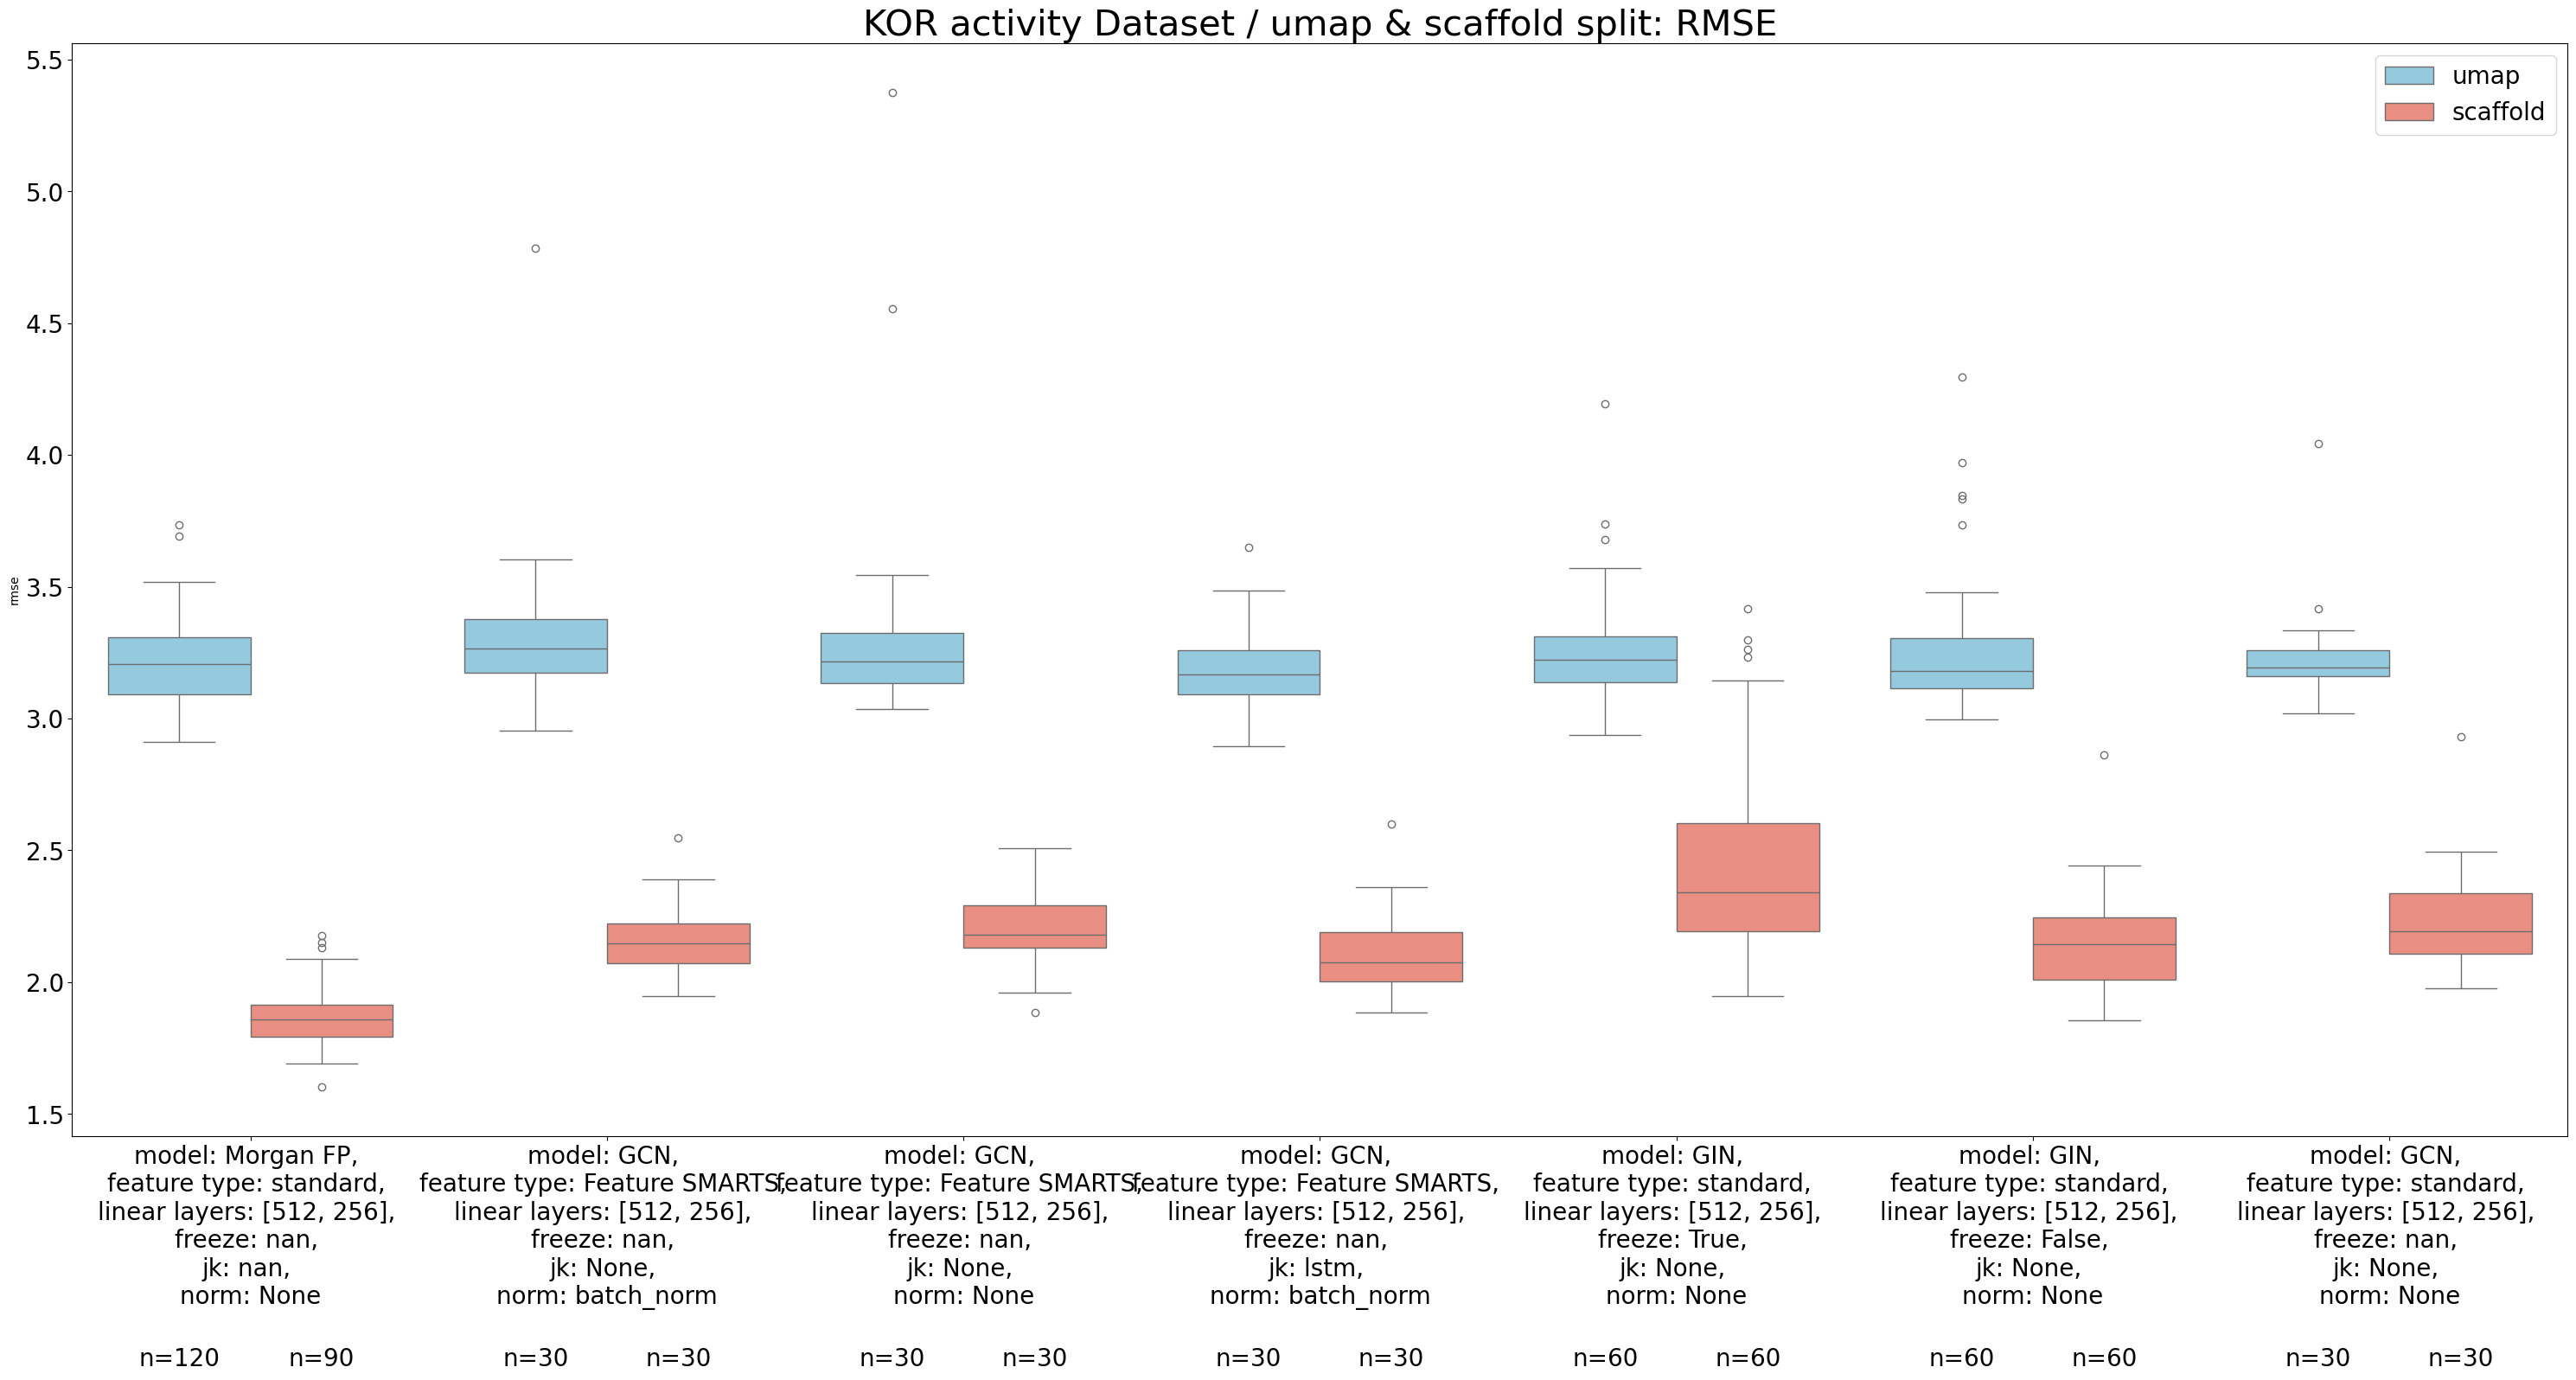
\includegraphics[width=1\linewidth]{umap_scaffold_comparison_kor_activity1.png}
    \caption{Enter Caption}
    \label{fig:enter-label}
\end{figure}

\section{Features and feature representation impact}

For other features, too, the usage of one-hot encoded versions could be more reasonable:

\section{Results for Jumping Knowledge, dropout, combined layers etc.}

The results for Jumping Knowledge are very inconsistent.
In some cases, jumping knowledge modes improve the results slightly, whereas in other variance is increased.

Commonly, batch norm increases performance consistently (except for architectures with frozen layers).
Optimized values for dropout (in the graph part as well as in the classifier) are often very high (even when batch norm is applied), indicating the importance of measures countering overfitting.



\section{Exotic Variations}

Furthermore, some variations of the general architecture consisting of a graph representation, in which atoms are represented as nodes and bonds as edges, and a final dense layer for classification have been tried out.
Even when they do not perform better than the architectures assessed in the previous chapter, a nearer investigations seems to be insightful. 

Similarly, the usage of a complete graph was tried.
Transformer and to the technique of inserting a supernode which is connected to all atoms of the graph representation \cite{Li.12.09.2017} and to the Graph convolution of Weave modules in which features from all pairs of atoms in the molecule are extracted \cite{Kearnes.2016}.

It also seems to be interesting to avoid the bipartite structure of graph representation and final classifier.
The graph channel size is subsequently decreased to 1. Since the output after the final graph layer has already size [1, batchsize], a further classification step is not necessary.

\subsection{Binary networks etc.}

\subsection{Incorporation of global properties}

\section{Custom Loss Functions}

The results so far have confirmed that outliers / activity cliffs play a crucial role.

Given these results, one could experiment with a dynamical version: Depending on the current size of the gradients, the alpha parameter will be modified.

(This is in particular true for some datasets from MoleculeNet which contain entries gathered from multiple publications in which not always the same experimental procedures were applied. This lack of standardization implies that the uncertainty of the reported values is much higher than the inherent error of the experimental setup alone.)


\subsection{Lipophilicity}

The results for the Lipophilicity dataset deviate in an interesting way.

In principle, the performance is very similar, but the lower variance of the GINs suggest their results are more stable. (Which outcome is preferable, depends on the practical purpose.)

Interestingly, in contrast to other datasets, the representation of the features (integer of one-hot encoding) seems to be crucial.

\subsection{Correlation between architectures}

Two related correlations are of interest, the predicted values itself and the residuals. 

Do such uneven splits lead to higher inter-run variance?

\section{Ensemble and Transfer learning}

The low correlation between runs with similar GNN architectures, in contrast to the rather large accordance for Molecular Fingerprints, probably is associated with the high inter-run variance even for the same architecture on the same data: Different runs lead to weight optimization which accurately predicts different data instances. This finding suggests that Ensemble learning, which has proven beneficial in many Deep Learning applications, could improve performance.

Transfer learning yields another opportunity to assess the importance of the trained parameters.
If they are ‚neutral‘, i.e. do not fit tightly to the task, but rather incorporate knowledge about physicochemical properties which can, in connection with an appropriate classifier, be used for different tasks.

(It is clear that this is not fully case: Given that float numbers, the probability is much more smaller. However, one can overcome this problem with the custom activation functions.)
For instance, on e can train it on one dataset use it for another which has the same or a related task.
Datasets which have the same properties (but within a different range), and totally different datasets.

For datasets with multiple properties (e.g., the ADME dataset), one could even try to create combined architectures which were trained on not only the property of interest, but also the other ones.

If GNNs really learn physicochemical properties (which are even of importance beyond the specific task), one should be able to increase performance by such an approach.

The ADME dataset is highly suited for such an investigation, because for many of the compounds several properties are listed, but for only a small subset all data is available.

\subsection{Carbohydrates}


Such compounds which consist solely of carbons (and hydrogens) are of special interest, since in this case the topology remains.
Thus, the layers have been investigated for such examples.


consisting of alkanes and fatty acids of different length.
\cite{Schweidtmann.2023}
Given that binary fingerprints should hardly be able to discern these structures, this is a good check for the reason of performance differences.


\subsection{Influcence of activity cliffs}

prediction error cliffs, i.e. molecules with a very similar objective value, but a high difference in error (for a specific ML/DL model). 

Fig
show interesting differences.

\subsection{Unique mapping of molecules}




\subsection{Subgraph GNNs}

An implementation using pygho has been adopted for the datasets used in this study.

For the ESOL dataset, this gives promising results.

Unfortunately, it is not trivial to adapt the code for processing nodes with multiple features.